\section{METHODOLOGY}
\label{sec:methodology}

\subsection{Preliminaries}
\label{subsec:preliminaries}

In this section, we formally define the notation and the recommendation problem addressed in this work.

Let $\mathcal{U} = \{ u_{1},u_{2},\ldots,u_{M}\}$ be the set of $M$ users and $\mathcal{V} = \{ v_{1},v_{2},\ldots,v_{N}\}$ be the set of $N$ items. We focus on the implicit feedback scenario, where user interactions are represented by a binary matrix $Y \in \{ 0,1\}^{M \times N}$. An entry $y_{uv} = 1$ indicates that user $u$ has interacted with item $v$ (e.g., purchased or clicked), while $y_{uv} = 0$ denotes unobserved interactions. For each user $u$, we denote the set of interacted items as $\mathcal{H}_{u} = \{ v \in \mathcal{V}|y_{uv} = 1\}$.

To support our Multi-Expert architecture, we model the data from three distinct views, corresponding to the inputs required by our Structural, Statistical, and Semantic experts:

\begin{itemize}
    \item \textbf{User-Item Graph}: We construct a bipartite graph $\mathcal{G} = \left( \mathcal{W},\mathcal{E} \right)$, where the node set $\mathcal{W} = \mathcal{U} \cup \mathcal{V}$ includes all users and items, and the edge set $\mathcal{E}$ corresponds to the observed interactions in $Y$. This graph serves as the foundation for our structural experts (e.g., StructCLR) to perform message passing.
    
    \item \textbf{Co-occurrence View (Statistical Signal)}: Beyond local connectivity, we consider the global item-item correlation. This is implicitly modeled by the item similarity matrix derived from $\mathbf{Y}^{T}\mathbf{Y}$, which captures the statistical co-occurrence patterns between items across the entire population. This view empowers our statistical experts (e.g., EASE, Tribe).
    
    \item \textbf{Semantic View (Content Signal)}: Each item $v$ is associated with a textual sequence $T_{v}$ (e.g., title, brand, description). This modality enables our semantic experts (e.g., BM25, UserKNN) and the LLM module to perform content-aware reasoning and denoising.
\end{itemize}

\textbf{Problem Definition (Top-K Recommendation)}. Given the interaction history $Y$ and item textual attributes $\{ T_{v}\}$, our goal is to learn a scoring function $f\left( u,v \right)$ that predicts the preference score of user $u$ for an unobserved item $v$. Based on these scores, we aim to distill a high-precision ranked list of $K$ items from the vast item space $\mathcal{V}$. This requires not only retrieving a broad set of relevant candidates (Expansion) but also rigorously filtering out structural noise to maximize information density in the top positions (Compression).

\begin{table}[htbp]
\centering
\caption{Notation Summary}
\label{tab:notation}
\begin{tabular}{ll}
\toprule
Symbol & Description \\
\midrule
$\mathcal{U},\mathcal{V}$ & Sets of users and items \\
$M,N$ & Number of users and items \\
$Y$ & User-item interaction matrix \\
$\mathcal{G}$ & User-item bipartite graph \\
$E_{u},E_{v}$ & Learned embeddings for user $u$ and item $v$ \\
$T_{v}$ & Textual content of item $v$ \\
$\mathcal{C}_{u}$ & The candidate item set retrieved by experts \\
$W_{\mathrm{pos}},W_{\mathrm{neg}}$ & Fusion weights for conditional RRF \\
\bottomrule
\end{tabular}
\end{table}

\subsection{Framework Overview}
\label{subsec:framework_overview}

To transcend the inherent limitations of single-view representations and effectively bridge the gap between collaborative signals and semantic reasoning, we propose ASC-Rec (Adaptive Structural-Semantic Cascade). As illustrated in Figure~\ref{fig:overview}, the proposed framework operates under an ``Expansion-Compression'' paradigm, treating the recommendation process as a progressive information distillation pipeline consisting of three stages:

\begin{figure}[htbp]
\centering
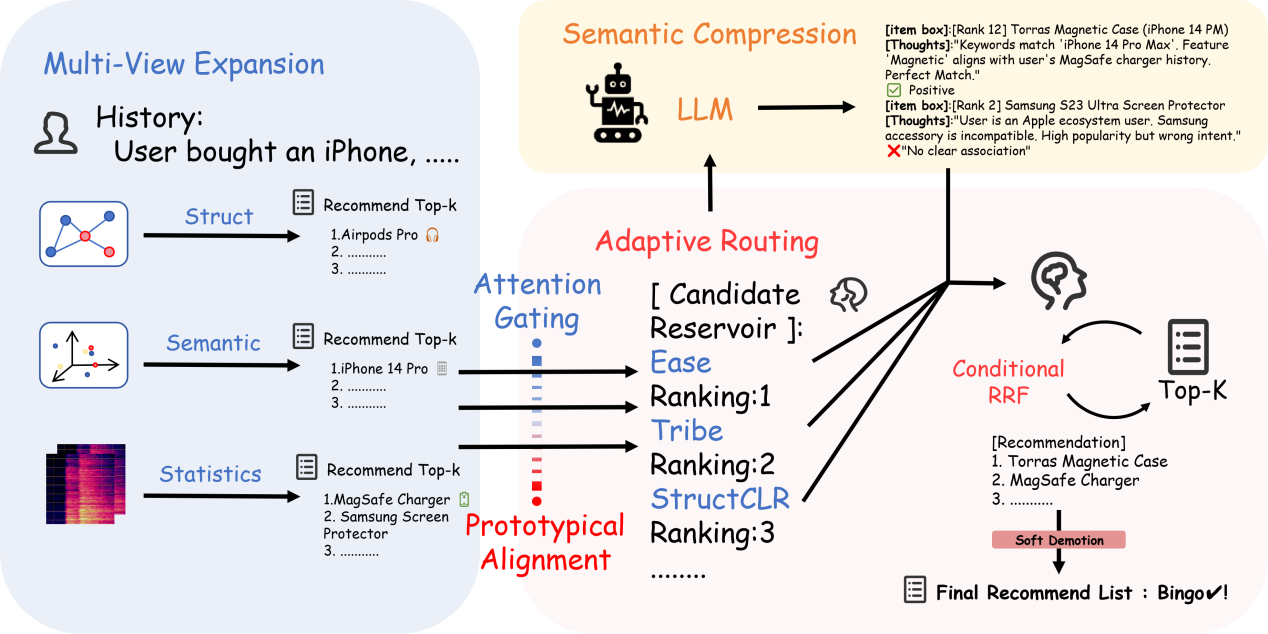
\includegraphics[width=0.95\textwidth]{figures/fig1_overview.png}
\caption{Framework overview of ASC-Rec. The system operates under an ``Expansion-Compression'' paradigm with three sequential stages: (1) Candidate Reservoir Construction via Multi-View Expert Pool, (2) Adaptive Routing for Structural Selection, and (3) Semantic Compression for Cognitive Refinement.}
\label{fig:overview}
\end{figure}

\begin{enumerate}
    \item \textbf{Candidate Reservoir Construction}: Recognizing that user intent is multifaceted and dynamic, we posit that relying on a single modality leads to suboptimal coverage. To address this, we construct a heterogeneous Expert Pool encompassing three distinct views: Structure, Statistics, and Semantics. This stage aims to maximize the Recall Upper Bound by aggregating diverse signals---ranging from high-order connectivity to keyword matching---thereby ensuring that the initial candidate pool covers the full spectrum of potential user interests.
    
    \item \textbf{Adaptive Routing (Structural Selection)}: Simple aggregation of experts often introduces noise and redundancy. To mitigate this, we introduce an Attention-based Dynamic Router. Acting as an adaptive gating mechanism, the Router computes user-specific importance weights based on the user's structural embedding. This stage functions as a ``Filter'', efficiently retrieving a high-quality candidate subset (e.g., Top-50) that aligns with the user's dominant behavioral pattern, effectively establishing a robust structural prior.
    
    \item \textbf{Semantic Compression (Cognitive Refinement)}: While the Router ensures high recall, the candidate list inevitably contains structurally plausible but semantically irrelevant noise (e.g., false positives due to popularity bias). In the final stage, we employ a Large Language Model (LLM) as a Semantic Compressor. By leveraging a novel Conditional Reciprocal Rank Fusion (Conditional RRF) strategy, the model incorporates semantic reasoning to identify and suppress negative candidates (``No clear association''). This process compresses the entropy of the ranking list, distilling valid items from the broad candidate pool into the ultra-head ranking positions (Top-K), thereby maximizing the utility within limited exposure slots.
\end{enumerate}

\subsection{Multi-View Expert Pool (Expansion Stage)}
\label{subsec:multi_view_expert_pool}

To ensure the initial candidate reservoir captures the full spectrum of user intent, we construct a heterogeneous expert pool $\mathcal{E}$. The design philosophy is governed by Mutual Complementarity: experts operate on orthogonal data views, ensuring that the scoring function $S_{k}\left( u,v \right)$ of the $k$-th expert covers the blind spots of others.

\subsubsection{Capturing Implicit Habits: The Structural View}

Graph-based and sequence-based models serve as the backbone of our system, excelling at capturing implicit user preferences from historical interactions $\mathcal{H}_{u}$.

\paragraph{StructCLR (Structural Expert):} Standard GCNs often suffer from noise and uniform embedding distribution. We propose StructCLR, an enhanced graph encoder. Unlike vanilla LightGCN, StructCLR introduces a temperature-scaled InfoNCE loss with explicit hard negative mining. By treating low-rated items (Rating $<$ 4) as hard negatives $\mathcal{N}_{\mathrm{hard}}$, we force the model to distinguish fine-grained preferences. The objective is defined as:

\begin{equation}
\mathcal{L}_{\mathrm{Struct}} = - \sum_{u \in \mathcal{U}}^{}\log\frac{\exp\left( e_{u} \cdot e_{v^{+}}/\tau \right)}{\sum_{i \in \mathcal{V}}^{}\exp\left( e_{u} \cdot e_{i}/\tau \right) + \beta\sum_{j \in \mathcal{N}_{\mathrm{hard}}}^{}\exp\left( e_{u} \cdot e_{j}/\tau \right)}
\end{equation}

where $\beta$ controls the penalty for confirmed negatives. The prediction score is computed as the inner product: $S_{\mathrm{struct}}\left( u,v \right) = e_{u}^{\top}e_{v}$. This provides a robust structural prior for the router.

\paragraph{SASRec (Sequence Expert):} To capture temporal dynamics, SASRec models the interaction sequence using self-attention. Given the history sequence $\mathcal{H}_{u}$, the prediction is based on the matching between the sequence representation $h_{L}$ and item embedding:

\begin{equation}
S_{\mathrm{seq}}\left( u,v \right) = h_{L}\left( \mathcal{H}_{u} \right)^{\top}e_{v}
\end{equation}

\subsubsection{Bridging Structural Gaps: The Statistical View}

Structural models struggle to connect items that are topologically distant or disjoint in the graph. We introduce statistical experts to bridge these structural gaps via global co-occurrence patterns.

\paragraph{EASE (Co-occurrence Expert):} While GCN propagates information locally, EASE captures the global item-item correlation matrix directly. It excels at identifying ``hard correlations'' (e.g., functional complements) that embedding-based models might miss due to the over-smoothing problem.

EASE computes a closed-form weight matrix $W \in \mathbb{R}^{N \times N}$ directly from the interaction matrix $Y$. It captures global item-item correlations by solving a constrained least-squares problem:

\begin{equation}
\min_{\mathbf{W}}\left\| \mathbf{Y} - \mathbf{YW} \right\|_{F}^{2} + \lambda\left\| \mathbf{W} \right\|_{F}^{2},\quad\mathrm{s.t.}\,\mathrm{diag}\left( \mathbf{W} \right) = 0
\end{equation}

The score is computed via sparse matrix multiplication: $S_{\mathrm{ease}}\left( u,: \right) = y_{u} \cdot W$.

\paragraph{Tribe (Cluster Expert):} To mitigate the noise from individual behaviors, we aggregate users into semantic clusters. This expert retrieves the most popular items within each ``Tribe,'' serving as a robust safety net against sparsity and overfitting. This expert clusters users into $K$ groups $\{ C_{1},\ldots,C_{K}\}$. For a user $u \in C_{k}$, the score is proportional to the item's popularity within the cluster:

\begin{equation}
S_{\mathrm{tribe}}\left( u,v \right) = \frac{\mathrm{Count}\left( v \in C_{k} \right)}{\sum_{v^{\prime}}^{}\mathrm{Count}\left( v^{\prime} \in C_{k} \right)}
\end{equation}

\subsubsection{Handling Explicit \& Cold-Start Intent: The Semantic View}

Both structural and statistical models fail when interaction data is scarce (Cold Start) or when user intent is explicitly content-driven. We address this by incorporating semantic experts.

\paragraph{BM25 (Search Expert):} Embedding models often suffer from ``semantic drift.'' BM25 ensures precision by performing rigid keyword matching between user history and item titles, capturing explicit search-like intents (e.g., specific brand or model requirements). We treat the user's history $\mathcal{H}_{u}$ as a query and item title $T_{v}$ as a document. The score represents the keyword matching degree:

\begin{equation}
S_{\mathrm{bm25}}\left( u,v \right) = \sum_{t \in \mathcal{H}_{u} \cap T_{v}}^{}\mathrm{IDF}\left( t \right) \cdot \frac{\mathrm{TF}\left( t,T_{v} \right) \cdot \left( k_{1} + 1 \right)}{\mathrm{TF}\left( t,T_{v} \right) + k_{1} \cdot \left( 1 - b + b \cdot \frac{\left| T_{v} \right|}{\mathrm{avgdl}} \right)}
\end{equation}

\paragraph{UserKNN (Semantic Expert):} This expert overcomes the ``Product Disjoint'' problem. By locating users with similar semantic profiles (averaged BERT embeddings) rather than overlapping purchase histories, it retrieves candidates from ``semantic soulmates,'' effectively handling scenarios where collaborative signals are weak. To handle disjoint item sets, we represent each user as the centroid of their historical item BERT embeddings: $c_{u} = \frac{1}{\left| \mathcal{H}_{u} \right|}\sum_{i \in \mathcal{H}_{u}}^{}\mathrm{BERT}\left( T_{i} \right)$. The score is aggregated from the top-$K$ semantic neighbors $\mathcal{N}_{u}^{\mathrm{sem}}$:

\begin{equation}
S_{\mathrm{knn}}\left( u,v \right) = \sum_{u^{\prime} \in \mathcal{N}_{u}^{\mathrm{sem}}}^{}\mathrm{Sim}\left( \mathbf{c}_{u},\mathbf{c}_{u^{\prime}} \right) \cdot \mathbb{I}\left( v \in \mathcal{H}_{u^{\prime}} \right)
\end{equation}

\subsection{Attention-based Dynamic Router}
\label{subsec:attention_router}

Given the heterogeneous expert pool $\mathcal{E} = \{ E_{1},\ldots,E_{M}\}$, a static aggregation strategy (e.g., averaging) is suboptimal because different users exhibit distinct behavioral patterns. For instance, a cold-start user may rely heavily on the BM25 (Search) expert, while a community-driven user aligns better with StructCLR (Structure).

To address this, we propose an Attention-based Dynamic Router that acts as an adaptive traffic controller. It learns to map a user's current state to the optimal expert combination.

\subsubsection{Expert Prototypes and Attention Mechanism}

We posit that each expert $E_{k}$ specializes in a specific subspace of user preferences. We learn a set of Expert Prototypes $P \in \mathbb{R}^{M \times d}$, where $p_{k}$ represents the latent centroid of users who are best served by expert $E_{k}$. We utilize the user embedding $e_{u}$ from the pre-trained StructCLR as the query vector, as it encodes the fundamental structural state of the user. The attention weight $\alpha_{u,k}$, representing the confidence assigned to expert $k$ for user $u$, is computed via a dot-product attention mechanism:

\begin{equation}
\alpha_{u,k} = \frac{\exp\left( \mathbf{e}_{u}^{\top}\mathbf{p}_{k}/\tau_{\mathrm{gate}} \right)}{\sum_{j = 1}^{M}\exp\left( \mathbf{e}_{u}^{\top}\mathbf{p}_{j}/\tau_{\mathrm{gate}} \right)}
\end{equation}

where $\tau_{\mathrm{gate}}$ is a temperature parameter to control the sparsity of the selection. A highly trusted expert receives a weight $\alpha_{u,k} \rightarrow 1$, while irrelevant experts are suppressed.

\subsubsection{Weighted Reservoir Construction}

Once the weights $\mathcal{A}_{u} = \{\alpha_{u,1},\ldots,\alpha_{u,M}\}$ are obtained, we generate the initial candidate reservoir $\mathcal{C}_{u}$. To combine the ranked lists from different experts (which may have vastly different score scales), we employ a Weighted Borda Count strategy. The aggregated score for an item $v$ is calculated as:

\begin{equation}
S_{\mathrm{router}}\left( u,v \right) = \sum_{k = 1}^{M}\alpha_{u,k} \cdot \frac{1}{\mathrm{rank}_{k}\left( v \right) + 1}
\end{equation}

Items are then sorted by $S_{\mathrm{router}}$, and the Top-$N$ (e.g., $N=50$) are selected to form the Candidate Reservoir passed to the next stage. This ensures that the reservoir is dominated by the most competent experts for the specific user $u$.

\subsubsection{Optimization with Oracle Supervision}

A key challenge in MoE is the ``collapse problem'' where the gate converges to a single expert. To prevent this, we employ a Supervised Gating strategy rather than end-to-end RL.

\textbf{Oracle Label Generation}: For each user $u$ in the validation set, we retrospectively evaluate which expert successfully retrieved the ground-truth item within the top ranks. We assign a ``best expert'' label $y_{u}^{\ast}$:

\begin{equation}
y_{u}^{\ast} = \arg\max_{k}\mathbb{I}\left( v_{\mathrm{truth}} \in \mathrm{TopK}\left( E_{k} \right) \right)
\end{equation}

\textbf{Training}: The Router is trained to predict this oracle label by minimizing the Cross-Entropy loss:

\begin{equation}
\mathcal{L}_{\mathrm{Router}} = - \sum_{u}^{}{\sum_{k = 1}^{M}\mathbb{I}}\left( y_{u}^{\ast} = k \right) \cdot \log\left( \alpha_{u,k} \right)
\end{equation}

This explicitly forces the Router to learn the correlation between user embeddings (state) and expert capabilities (action).

\subsection{LLM-driven Semantic Compression}

While the Router effectively maximizes the recall upper bound (Expansion), the candidate reservoir $\mathcal{C}_{u}$ inevitably contains ``Retrieval Noise''---candidates that are retrieved due to statistical correlations or keyword overlaps but are functionally irrelevant to the user's specific intent (e.g., false positives caused by popularity bias).

To address this, we propose a Semantic Compression module. Unlike traditional reranking, this module functions as a ``Denoising Filter''. It leverages the reasoning capability of LLMs to identify these false positives and applies a Conditional Reciprocal Rank Fusion (Conditional RRF) strategy to suppress noise without discarding valid signals established by the Router.

\subsubsection{Context-Aware Reasoning Generation}

Directly asking LLMs to output a ranking score often leads to poor calibration. Instead, we adopt a ``Generate-then-Discriminate'' paradigm. We employ GLM-4.6 as a Reasoning Generator to produce a textual rationale $R_{uv}$ for each user-item pair.

To ground the LLM's reasoning and mitigate hallucinations, we inject ``Source Context'' into the prompt. We explicitly inform the LLM which expert retrieved the item (e.g., ``Matched by BM25'' or ``Recommended by StructCLR'').

\begin{itemize}
    \item \textbf{Prompting Strategy}: We utilize Few-Shot Chain-of-Thought (CoT) prompting. The LLM is instructed to act as a strict auditor.
    \item \textbf{Negative Detection}: Crucially, we instruct the LLM to output a specific flag token (e.g., ``No clear association'') if the item is semantically incompatible with the user's history.
\end{itemize}

\subsubsection{Discriminative Semantic Scoring}

To quantify the generated rationales, we utilize a fine-tuned Cross-Encoder (BGE-Reranker) as the Discriminator. The discriminator computes a semantic relevance score $S_{\mathrm{sem}}\left( u,v \right)$ by jointly encoding the user history $\mathcal{H}_{u}$ and the item profile augmented with the generated rationale:

\begin{equation}
S_{\mathrm{sem}}\left( u,v \right) = \sigma\left( \mathrm{CrossEncoder}\left( \mathcal{H}_{u},T_{v} \oplus \left[ \mathrm{SEP} \right] \oplus R_{uv} \right) \right)
\end{equation}

where $\oplus$ denotes concatenation. By conditioning the score on the generated rationale $R_{uv}$, the discriminator can distinguish between ``strong recommendations'' and ``weak recommendations''.

\subsubsection{Conditional RRF with Soft Demotion}

A critical challenge in LLM-based recommendation is the False Negative problem. Our empirical analysis reveals that LLMs may erroneously reject implicitly correlated items (e.g., functional complements found by EASE) due to a lack of collaborative knowledge.

To solve this, we propose a Conditional RRF strategy with an Asymmetric Weighting Mechanism. We fuse the base rank from the Router $\left( \mathrm{rank}_{\mathrm{router}} \right)$ and the semantic rank from the Cross-Encoder $\left( \mathrm{rank}_{\mathrm{sem}} \right)$ as follows:

\begin{equation}
S_{\mathrm{final}}\left( u,v \right) = \underbrace{\frac{1.0}{\eta + \mathrm{rank}_{\mathrm{router}}}}_{\mathrm{Router\ Prior}} + \underbrace{\frac{\lambda}{\eta + \mathrm{rank}_{\mathrm{sem}}}}_{\mathrm{Semantic\ Adjustment}}
\end{equation}

where $\eta$ is a smoothing constant (e.g., 60). The semantic weight $\lambda$ is dynamic, conditioned on the sentiment of the rationale $R_{uv}$:

\begin{equation}
\lambda = \begin{cases}
w_{\mathrm{pos}} & \text{if } R_{uv} \text{ is Positive} \\
w_{\mathrm{neg}} & \text{if } R_{uv} \text{ is Negative (``No clear association'')}
\end{cases}
\end{equation}

\begin{itemize}
    \item \textbf{Positive Boost} ($w_{\mathrm{pos}}=0.5$): When the LLM identifies a clear semantic match, we amplify its score to promote the item to the top.
    \item \textbf{Soft Demotion} ($w_{\mathrm{neg}}=0.3$): When the LLM flags an item as irrelevant, we assign a lower weight but do not zero it out. This implements a ``Soft Demotion'' strategy: if an item has a very high priority in the Router (indicating strong collaborative or statistical evidence), the robust Router Prior ensures it remains in the recommendation list, protecting against LLM misjudgment. Conversely, if an item is both statistically weak and semantically irrelevant, it naturally sinks to the bottom.
\end{itemize}

This mechanism effectively compresses the information entropy, distilling the candidate list to a high-density state where top-ranked items satisfy both multi-view retrieval criteria and semantic coherence.